\documentclass[border=0.2cm]{standalone}
\usepackage{pgfplots}
\pgfplotsset{compat=1.18}

% Define custom colors
\definecolor{customcolor1}{RGB}{58, 164, 250}  % Blue for bars

\begin{document}

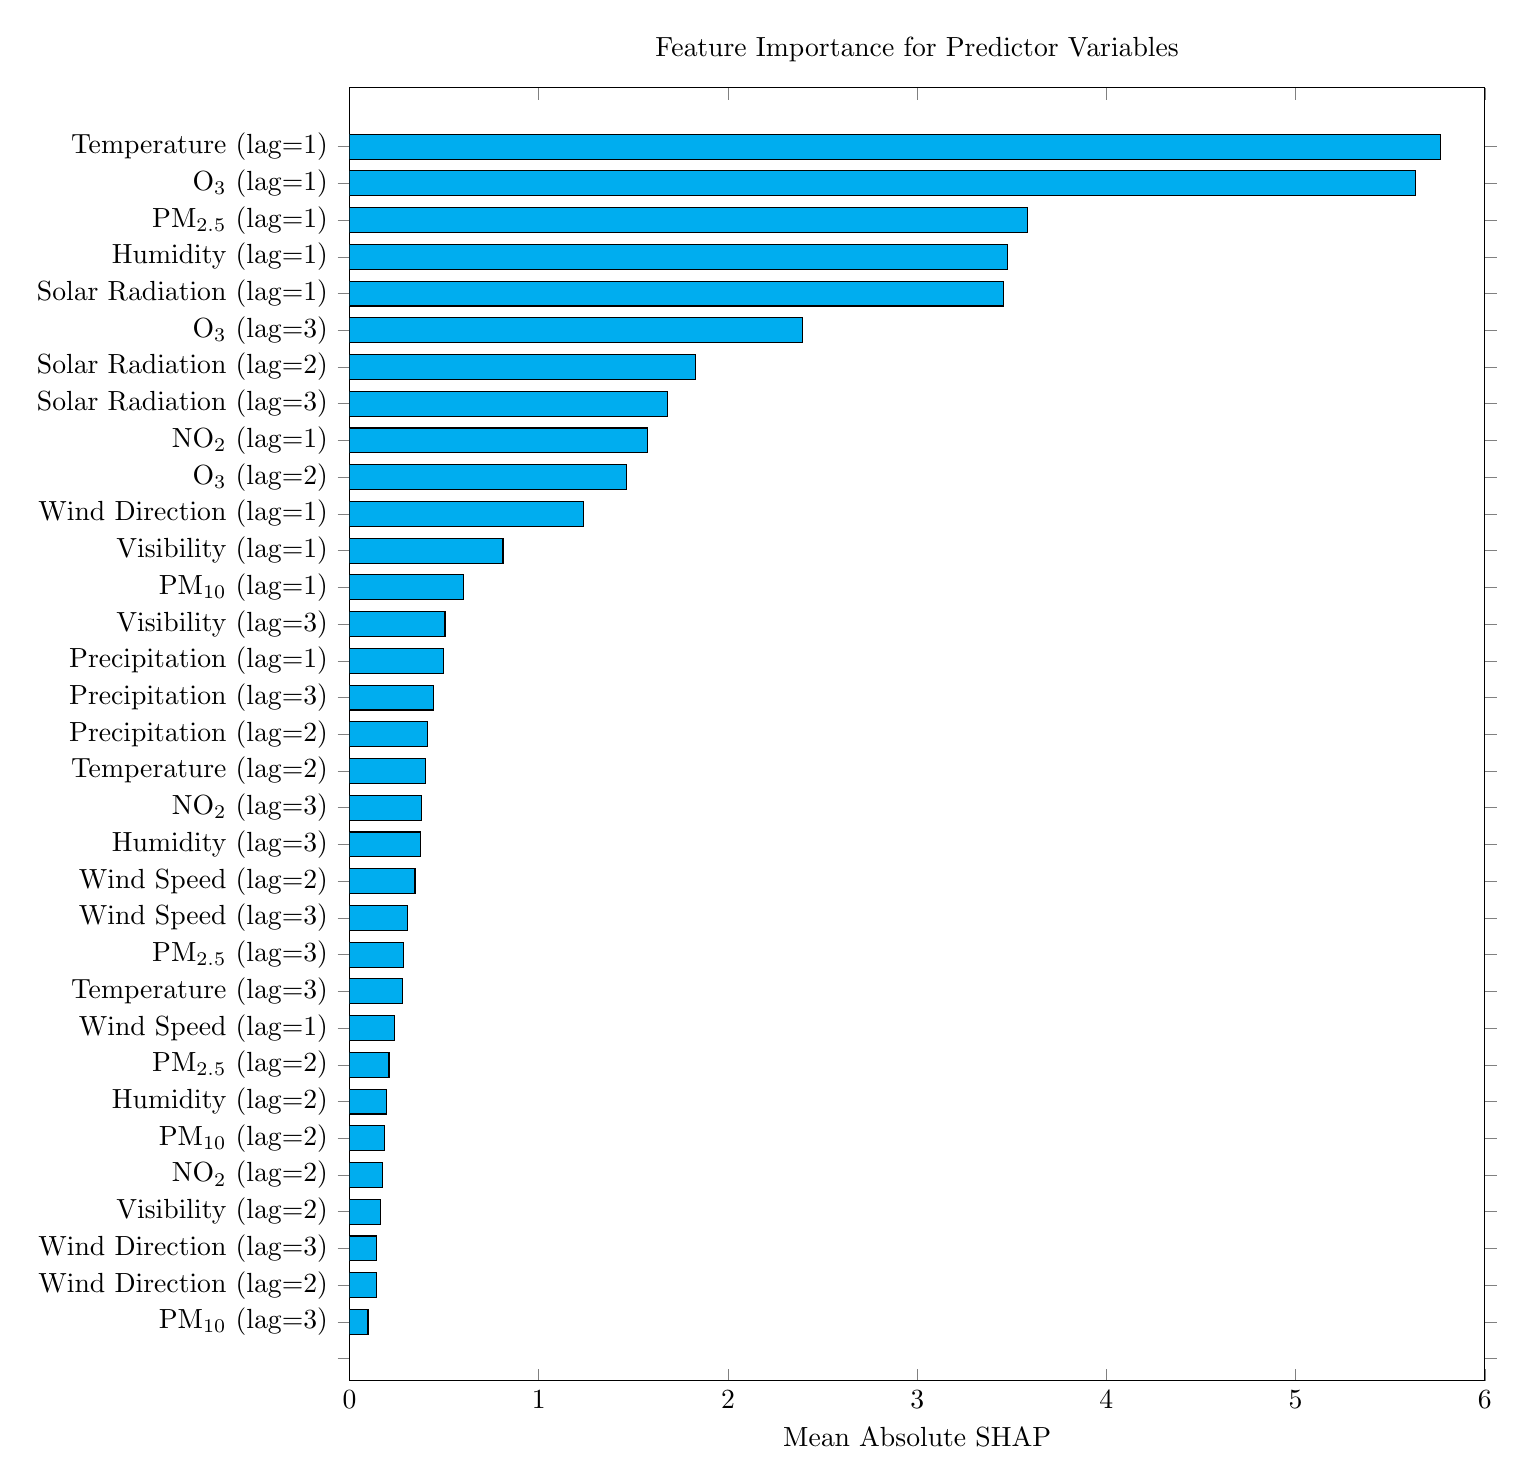
\begin{tikzpicture}

\begin{axis}[
    xbar, % Horizontal bars
    bar width=9pt, % Narrower bars
    xmin=0, 
    xmax=6, 
    title={Feature Importance for Predictor Variables},
    xlabel={Mean Absolute SHAP},
    ytick={0,1,...,33},
    yticklabels={
        Temperature (lag=1), O$_3$ (lag=1), PM$_{2.5}$ (lag=1), Humidity (lag=1), Solar Radiation (lag=1), O$_3$ (lag=3), Solar Radiation (lag=2), Solar Radiation (lag=3), NO$_2$ (lag=1), O$_3$ (lag=2),
        Wind Direction (lag=1), Visibility (lag=1), PM$_{10}$ (lag=1), Visibility (lag=3), Precipitation (lag=1), Precipitation (lag=3), Precipitation (lag=2), Temperature (lag=2), NO$_2$ (lag=3), Humidity (lag=3), 
        Wind Speed (lag=2), Wind Speed (lag=3), PM$_{2.5}$ (lag=3), Temperature (lag=3), Wind Speed (lag=1), PM$_{2.5}$ (lag=2), Humidity (lag=2), PM$_{10}$ (lag=2), NO$_2$ (lag=2), Visibility (lag=2), 
        Wind Direction (lag=3), Wind Direction (lag=2), PM$_{10}$ (lag=3)
    },
    xtick={0,1,2,3,4,5,6}, % Set x ticks
    enlarge y limits=0.05, % Increase space between bars
    y dir=reverse, % Reverse y-direction so labels appear in correct order
    width=16cm,
    height=18cm, % Adjust height for more spacing
    ytick distance=1, % Increase vertical spacing between rows
]

% Plot the importance values
\addplot[fill=cyan] coordinates {
    (5.766941,0) (5.63263,1) (3.5815392,2) (3.475367,3) (3.456865,4) 
    (2.3959482,5) (1.8265718,6) (1.6795981,7) (1.5732919,8) (1.464834,9) 
    (1.2373743,10) (0.8109572,11) (0.60146403,12) (0.5048162,13) (0.49500573,14) 
    (0.44572872,15) (0.41351405,16) (0.4023266,17) (0.38021353,18) (0.3769183,19) 
    (0.3461746,20) (0.3079201,21) (0.285651,22) (0.28092846,23) (0.23774858,24) 
    (0.20836349,25) (0.1959943,26) (0.18470103,27) (0.1738453,28) (0.16350256,29) 
    (0.14222378,30) (0.14136884,31) (0.09763571,32)
};

\end{axis}

\end{tikzpicture}

\end{document}
